%% LaTeX Beamer presentation template (requires beamer package)
%% see http://latex-beamer.sourceforge.net/
%% idea contributed by H. Turgut Uyar
%% template based on a template by Till Tantau
%% this template is still evolving - it might differ in future releases!

\documentclass[hyperref={pdfpagelabels=false}]{beamer}

\mode<presentation>

\usepackage{graphicx}
\usetheme{isu}
\usepackage{times}
\usepackage{amsmath,amsthm, amssymb, latexsym}
\boldmath
\usepackage[english]{babel}
\usepackage[latin1]{inputenc}

\usepackage{natbib}
\bibliographystyle{apalike}

\DeclareGraphicsExtensions{.pdf,.jpg,.png}
\graphicspath{{figures/}}

\title[Proposal]{
    A Tale of Two Language Models:\linebreak
    Formally Validating Pig Compilation Algorithm
}
\author[Team Axum: David Johnston and Bijon Bose]{Team Axum: David Johnston and Bijon Bose}
\institute[ISU]{
    Department of Computer Science \linebreak
    Iowa State University\linebreak
    dwtj@iastate.edu\linebreak
    bkbose@iastate.edu
}\date[COMS 641]{COMS 641: Data Intensive Languages and Systems - Design and Semantics}
%\date{Month X, 20XX}


% If you have a file called "university-logo-filename.xxx", where xxx
% is a graphic format that can be processed by latex or pdflatex,
% resp., then you can add a logo as follows:

%\pgfdeclareimage[height=0.25cm]{logo}{figures/logo}
%\logo{\pgfuseimage{logo}}


\begin{document}
  \begin{frame}[plain]
    \titlepage
  \end{frame}

  \section*{Overview}

\begin{frame}
\begin{itemize}
  \item The Problem
  \begin{itemize}
    \item Correctness of Pig programs depends upon correctness of compilation
          from Pig semantic model to the MapReduce semantic model.
  \end{itemize}

  \item Our Approach
  \begin{itemize}
    \item Coq: Formally model languages, semantics, compilation models; make
          correctness/equivalency proofs.
  \end{itemize}

  \item Evaluation
  \begin{itemize}
    \item Coq: Successfully write correctness proofs.
  \end{itemize}

  \item Benefits
  \begin{itemize}
    \item Formalization of both Pig and MapReduce semantic models can be reused.
    \item More advanced (i.e. optimizing) compilation algorithms can be modeled
          and validated.
  \end{itemize}

\end{itemize}
\end{frame}

  \section{The Problem}
%\begin{frame}
%  \frametitle{Course Rationale: Prevent This Class of Errors}
%  \begin{quote}
%      Language and framework-specific errors, i.e. errors that arise due to
%      incorrect understanding of the semantics of the language and/or framework
%      and its guarantees.
%  \end{quote}
%\end{frame}

\begin{frame}
  \frametitle{The Problem: Program Correctness Depends Upon Compilation
    Correctness}
  \begin{enumerate}
    \item Programs written in sequential, declarative style PigLatin are compiled to distributed Hadoop MapReduce jobs.
    \item A Pig program's correctness requires correct compilation.
    \item Correct compilation depends upon a non-trivial mapping from
      properties over Pig semantics to properties over MapReduce semantics through the transformation into Logical Plan and Physical Plan.
    \item Our goal is to prove the correctness of this compilation.
  \end{enumerate}
\end{frame}

  \section{Our Approach}

\subsection{Pig Latin Features}
\begin{frame}{Features}
\begin{itemize}
	\item DataFlow Language:
	\begin{itemize}
		\item Programmer defines a sequence of statements where each carries out a single 					  data transformation. The output relation of each statement is stored in an  					  identifier to be used later in the program.
	\end{itemize}
	\item User Defined Functions:
	\begin{itemize}
		\item User defined functions provide the flexibility to perform specialized data 				 	  processing tasks.
	\end{itemize}
	\item Abstract Parallelism:
	\begin{itemize}
		\item Pig Latin programs are represented a sequential way to define the query 					      statements abstracting away the underlying parallelism performed through the 					  map-reduce tasks.
	\end{itemize}
\end{itemize}
\end{frame}

\subsection{Formalism}
\begin{frame}{Four Stages of Pig Programs}
\begin{itemize}
	\item A Pig Latin program passes through four stages of compilation:
	\begin{itemize}
		\item Pig Latin Program
		\item Logical Plan
		\item Physical Plan
		\item Map Reduce Phase
	\end{itemize}
	\item The logical plan is an one-to-one mapping from Pig Latin Program and the in Map-				  Reduces phase is executed by assigning physical operators to corresponding map-				  reduce jobs. So we've started our formalism by defining the calculus for Logical 				  plan and Map-Reduce in terms of Pig Latin programs.
\end{itemize}
\end{frame}

\subsection{Formalism for Logical Plan}

\begin{frame}{Conventions}
\centering
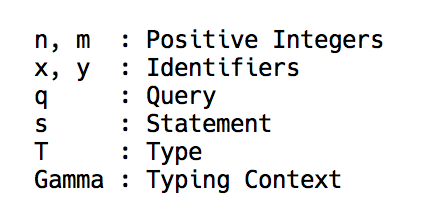
\includegraphics[scale=0.80]{conventions}
\end{frame}

\begin{frame}{Grammar: Queries}
\centering
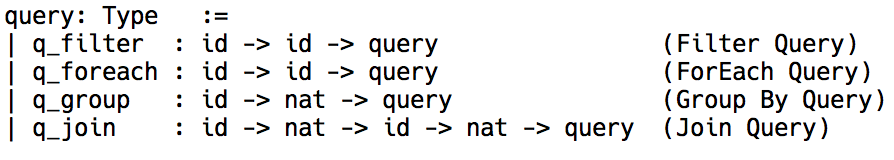
\includegraphics[scale=0.60]{query}
\end{frame}

\begin{frame}{Grammar: Statements}
\centering
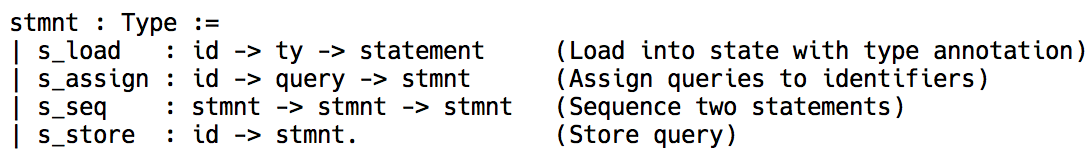
\includegraphics[scale=0.60]{stmnt}
\end{frame}

\begin{frame}{Types}
\centering
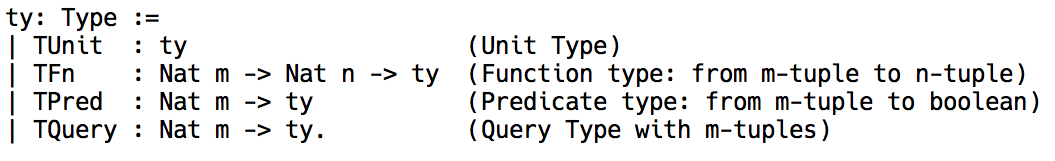
\includegraphics[scale=0.60]{ty}
\end{frame}

\begin{frame}{Typing Rules: Queries}
\centering
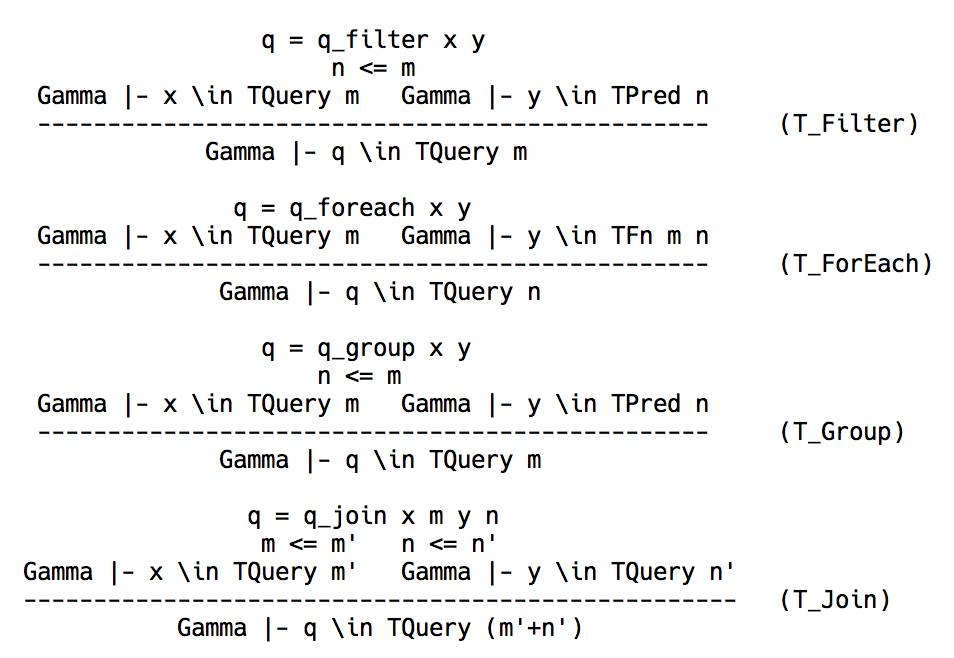
\includegraphics[scale=0.50]{T_Queries}
\end{frame}

\begin{frame}{Typing Rules: Statements}
\centering
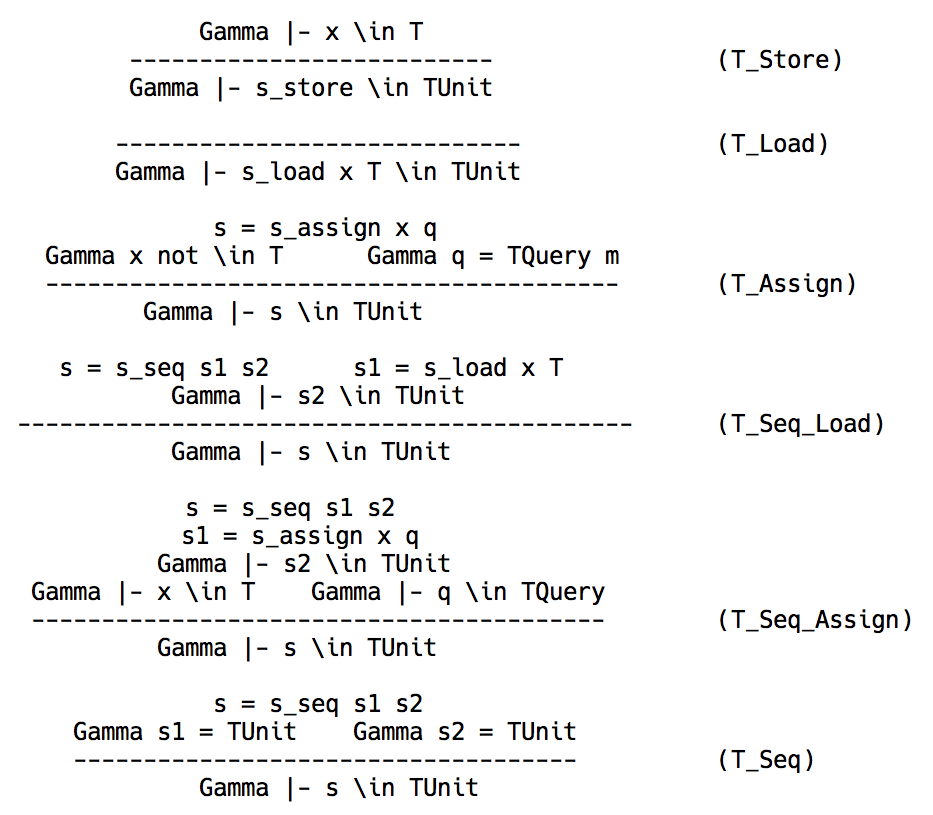
\includegraphics[scale=0.40]{T_Statements}
\end{frame}

  \section{Evaluation}

\begin{frame}
% TODO Include graphs/charts for your evaluation
\end{frame}

  \section*{}

%\textsc{\textsc{\textsc{\begin{frame}{Future Work}
  %\begin{itemize}
    %\item % TODO Talk about future work/limitations here
  %\end{itemize}
%\end{frame}


%\begin{frame}{Conclusion}
% TODO copy/paste overview here (from intro.tex)
%\end{frame}}


\begin{frame}
\begin{beamercolorbox}[center]{white}
  {\Large Questions?}

  \vspace{2em}\hfill

  \url{https://github.com/isu-cs641s16-axum}
\end{beamercolorbox}
\end{frame}


  \appendix

% make sure you have a blank slide in case you accidentally go past your conclusion
\begin{frame}[plain]
\end{frame}


% these slides are to help answer potential questions and generally arent shown
% unless needed or there is extra time
\begin{frame}[plain]{Hidden Slide 1}
\end{frame}

\begin{frame}[plain]{Hidden Slide 2}
\end{frame}


  \begin{frame}[allowframebreaks]
    \bibliography{refs}{}
  \end{frame}
\end{document}
